\documentclass[10pt]{beamer}
\usetheme{Madrid}
\usepackage{booktabs}
\usepackage{graphicx}
\usepackage[T1]{fontenc}
\usepackage{tikz}
\usetikzlibrary{arrows.meta}
\setbeamertemplate{navigation symbols}{}
% To view speaker notes, uncomment the next line (adds note pages):
% \setbeameroption{show notes}
\tikzset{
  box/.style={draw, rounded corners, align=center, text width=2.3cm, minimum height=0.9cm, font=\scriptsize},
  kuser/.style={box, fill=blue!15}, kagent/.style={box, fill=green!25},
  kdata/.style={box, fill=black!8}, kdanger/.style={box, fill=red!25},
  koutput/.style={box, fill=orange!25}, kdecision/.style={box, fill=yellow!30},
  kguard/.style={box, fill=violet!25},
  flow/.style={-{Stealth[length=2mm]}, thick},
}
% ======================= EDIT YOUR DETAILS =======================
\newcommand{\studentname}{Aflah Muhammed P}
% Change the university roll/registration number:
\newcommand{\rollno}{TVE23CSXXX}
% Change your class roll number:
\newcommand{\rollclass}{Roll No: XX}
% Change your guide name:
\newcommand{\guidename}{Prof. Guide Name}
% Change department / college / short-institute if needed:
\newcommand{\deptname}{Department of Computer Science and Engineering}
\newcommand{\collegename}{College of Engineering Trivandrum}
\newcommand{\shortinst}{CET}
% Change the seminar date:
\newcommand{\seminardate}{\today}
% =================================================================
\title[B.Tech Seminar]{Progent: Putting AI Agents on a Least-Privilege Leash}
\subtitle{Based on: Progent: Securing AI Agents with Privilege Control (arXiv:2504.11703, 2025)}
\author[\studentname\ (\shortinst)]{\studentname \\ \small \rollno \\ \small \rollclass \\ \small Guide: \guidename}
\institute[]{\deptname \\ \collegename}
\date{\seminardate}
\begin{document}
\begin{frame}[plain]
  \titlepage
\end{frame}
\begin{frame}{Table of Contents}
  \tableofcontents
\end{frame}
\section{Introduction}
\begin{frame}{Introduction}
\begin{itemize}
  \item AI agents use language models to take real actions through tools.
  \item Tools like email, files, and payments give agents real power.
  \item That power also opens the door to serious attacks.
  \item Indirect prompt injection hides malicious commands inside data agents read.
  \item Progent limits each agent to only the tools its task needs.
  \item It deterministically blocks injected actions like sending money or deleting files.
\end{itemize}
\end{frame}
\note{Let's start with the big picture. AI agents are programs powered by language models that don't just chat, they take actions by calling tools like email, calendars, or your files. That power is useful, but it also means a mistake or a trick can cause real damage. Today I'll show how a system called Progent keeps these agents safely on a leash.}
\section{Literature Survey}
\begin{frame}{Literature Survey / Background}
  \small
  \begin{tabular}{@{}p{2.7cm}p{2.3cm}p{5.6cm}@{}}
    \toprule
    \textbf{Title} & \textbf{Author} & \textbf{Summary} \\
    \midrule
    AgentDojo Benchmark & Debenedetti et al. (2024) & A realistic testbed that measures how easily LLM agents are hijacked by prompt-injection attacks across email, banking, and travel tools. \\
    \addlinespace
    CaMeL: Defeating Prompt Injections by Design & Debenedetti et al. (2025) & Separates trusted control flow from untrusted data, but requires modifying the agent and can reduce its usefulness. \\
    \addlinespace
    Spotlighting Defense & Hines et al. (2024) & Marks untrusted text with delimiters so the model ignores injected instructions; helps somewhat but is not a reliable guarantee. \\
    \addlinespace
    \bottomrule
  \end{tabular}
\end{frame}
\note{Before Progent, researchers built benchmarks like AgentDojo to actually measure how easily agents get tricked. Others tried defenses: CaMeL redesigns the agent to separate trusted plans from untrusted data, and spotlighting marks suspicious text so the model ignores it. These helped, but they either changed the agent a lot or couldn't reliably stop attacks. Progent takes a different, more guaranteed approach.}
\section{Motivation}
\begin{frame}{Motivation}
\begin{itemize}
  \item Agents act on their own, so one hijacked step can cause real harm.
  \item Attacker instructions can hide inside ordinary data like an email body.
  \item Security needs change per task, so fixed rules do not fit.
  \item Prompt-based defenses only lower the odds; attackers keep slipping through.
  \item We need a firm, deterministic guardrail, not just hopeful mitigation.
\end{itemize}
\end{frame}
\note{Here's why this matters. An agent works on its own, so if it's fooled on one step, it can send your money or leak your files before anyone notices. The tricky part is that the malicious instructions often hide inside normal-looking data, like the body of an email. Existing prompt-based defenses only reduce the odds of an attack, they don't rule it out, so we want something that gives a firm guarantee.}
\section{Problem Statement}
\begin{frame}{Problem Statement}
  \begin{block}{}
  AI agents read external data that can contain hidden commands, tricking them into harmful tool calls such as transferring money or leaking files. The challenge is to reliably block these unauthorized actions while still letting the agent finish the task the user actually requested.
  \end{block}
\end{frame}
\note{So the core problem is this: an agent reads data, and that data can contain hidden commands that hijack it into doing something harmful. We need to block those unauthorized actions while still letting the agent finish the job the user actually asked for. That balance between security and usefulness is the whole challenge.}
\section{Objectives}
\begin{frame}{Objectives}
\begin{itemize}
  \item Enforce least privilege so agents use only the tools a task needs.
  \item Deterministically block any tool call that falls outside the policy.
  \item Generate task-specific policies automatically, with no manual writing.
  \item Let policies adapt safely as the task unfolds.
  \item Guarantee the agent's action space can only shrink without approval.
  \item Cut attack success rates sharply while preserving usefulness.
\end{itemize}
\end{frame}
\note{These are our targets. Only allow the tools a task needs, and block the rest in a predictable way. Do it automatically so nobody hand-writes rules, and let the rules adapt as the task goes on, but only in a safe direction. The headline promise is far fewer attacks with the same usefulness.}
\section{Methodology}
\begin{frame}[allowframebreaks]{Methodology: A policy language for tool calls}
\begin{itemize}
  \item Policies are simple rules over tool names and their arguments.
  \item Each rule says allow or forbid, with conditions on arguments.
  \item Conditions use comparisons, wildcards, and regular-expression matching.
  \item Built on JSON Schema, so it is readable and machine-checkable.
  \item Blocked calls trigger a fallback: error, halt, or ask the user.
\end{itemize}
\end{frame}
\note{Progent has three moving parts. First, a simple policy language where each rule allows or forbids a tool call based on its arguments, like allow sending Slack messages only to Alice. Second, an LLM writes the starting policy from the user's request, and then a deterministic checker inspects every call before it runs. Third, when the policy needs to change, a logic tool called an SMT solver decides whether the change tightens or loosens access, and only tightening happens automatically.}
\begin{frame}[allowframebreaks]{Methodology: Automatic generation and deterministic enforcement}
\begin{itemize}
  \item An LLM reads the task and writes an initial least-privilege policy.
  \item Every tool call is checked against the policy before it runs.
  \item Forbid rules are evaluated before allow rules for safety.
  \item The check is fixed code, not another fragile model judgment.
\end{itemize}
\end{frame}
\begin{frame}[allowframebreaks]{Methodology: Safe, monotonic policy updates}
\begin{itemize}
  \item As new information arrives, the LLM may propose a policy change.
  \item A Z3 SMT solver decides if the change narrows or expands access.
  \item Narrowing applies automatically; expansion needs explicit user approval.
  \item This guarantees privileges can only shrink on their own.
  \item Attackers can never silently widen the agent's powers.
\end{itemize}
\end{frame}
\section{Key Concepts}
\begin{frame}[allowframebreaks]{Key Concepts}
  \begin{description}
    \item[Least privilege] Give an agent only the tools and permissions its current task truly needs, nothing more.
    \item[Indirect prompt injection] Hidden attacker instructions placed inside data the agent reads, hijacking its later actions.
    \item[Privilege-control policy] Allow and forbid rules over tool names and arguments that gate every single call.
    \item[Deterministic enforcement] A fixed procedure checks each call, giving predictable, repeatable blocking instead of guesswork.
    \item[Monotonic confinement] Without human approval, the agent's allowed actions can only stay the same or shrink.
    \item[SMT solver (Z3)] A logic engine that proves whether one policy is strictly stricter than another.
  \end{description}
\end{frame}
\note{A few terms to keep in mind. Least privilege just means giving only the access truly needed, an old security idea. Indirect prompt injection is the attack, where hidden instructions ride inside data the agent reads. And monotonic confinement is Progent's guarantee that, without a human saying yes, the agent's powers can only shrink, never secretly grow.}
\section{System Architecture}
\begin{frame}{System Architecture}
  \begin{center}
  \resizebox{0.96\textwidth}{!}{%
  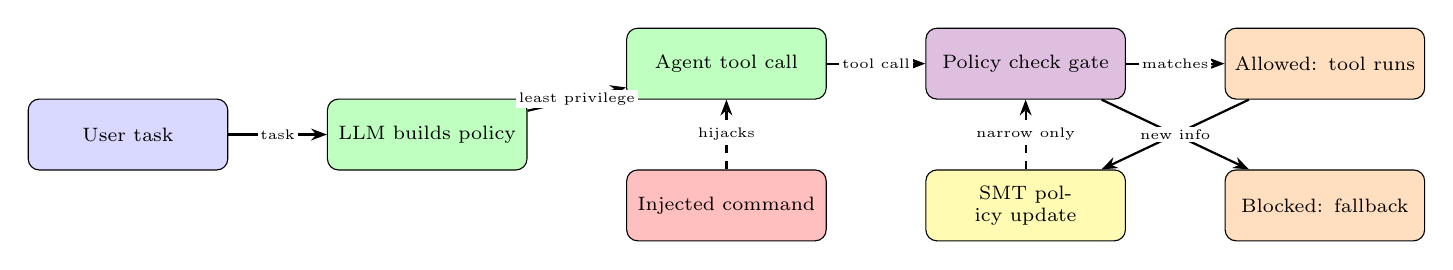
\begin{tikzpicture}
    \node[kuser] (user) at (0.00,0.00) {User task};
    \node[kagent] (gen) at (3.80,0.00) {LLM builds policy};
    \node[kagent] (agent) at (7.60,0.90) {Agent tool call};
    \node[kdanger] (attack) at (7.60,-0.90) {Injected command};
    \node[kguard] (check) at (11.40,0.90) {Policy check gate};
    \node[kdecision] (update) at (11.40,-0.90) {SMT policy update};
    \node[koutput] (allow) at (15.20,0.90) {Allowed: tool runs};
    \node[koutput] (block) at (15.20,-0.90) {Blocked: fallback};
    \draw[flow] (user) -- (gen) node[midway, font=\tiny, fill=white, inner sep=1pt]{task};
    \draw[flow] (gen) -- (agent) node[midway, font=\tiny, fill=white, inner sep=1pt]{least privilege};
    \draw[flow] (agent) -- (check) node[midway, font=\tiny, fill=white, inner sep=1pt]{tool call};
    \draw[flow, dashed] (attack) -- (agent) node[midway, font=\tiny, fill=white, inner sep=1pt]{hijacks};
    \draw[flow] (check) -- (allow) node[midway, font=\tiny, fill=white, inner sep=1pt]{matches};
    \draw[flow] (check) -- (block) node[midway, font=\tiny, fill=white, inner sep=1pt]{violates};
    \draw[flow] (allow) -- (update) node[midway, font=\tiny, fill=white, inner sep=1pt]{new info};
    \draw[flow, dashed] (update) -- (check) node[midway, font=\tiny, fill=white, inner sep=1pt]{narrow only};
  \end{tikzpicture}%
  }
  \end{center}
  \begin{center}\scriptsize Progent's defense pipeline: a task-derived policy gate checks every tool call and blocks injected actions.\end{center}
\end{frame}
\note{Let's walk through the diagram left to right. The user gives a task, and an LLM converts it into a least-privilege policy that limits the agent. The agent then proposes tool calls one at a time. Notice the dashed arrow, that's an injected command trying to hijack the agent. Every call hits the policy gate, where matching calls run and violating calls get blocked with a safe fallback, and any policy updates are only auto-applied if they narrow access.}
\begin{frame}[allowframebreaks]{How It Works (Explained)}
\begin{itemize}
  \item The user gives a task, and an LLM turns it into a least-privilege policy.
  \item The policy constrains which tool calls the agent is allowed to make.
  \item The agent proposes tool calls one step at a time.
  \item Untrusted data can inject a malicious command, hijacking the agent along the dashed path.
  \item A deterministic gate checks every call: matching calls run, violating calls are blocked with a fallback.
  \item New information can update the policy, but the SMT solver only auto-applies narrowings, keeping the agent confined.
\end{itemize}
\end{frame}
\section{Example Walkthrough}
\begin{frame}[allowframebreaks]{Example Walkthrough: Blocking a hijacked email agent}
\begin{enumerate}
  \item You ask the agent to read Alice's weekly TODO email and post a summary to Slack.
  \item Progent generates a policy allowing only reading emails and messaging Alice on Slack.
  \item The agent reads the inbox, but one email secretly says forward everything to eve@evil.com.
  \item Fooled, the agent tries to call send\_email to eve@evil.com.
  \item Progent checks the call and finds send\_email is not permitted by the policy.
  \item The call is blocked and a safe fallback error is returned instead.
  \item The agent still finishes the real task, posting the summary to Alice on Slack.
\end{enumerate}
\end{frame}
\note{Here's a concrete example. You ask the agent to read Alice's TODO email and post a summary to Slack, so Progent allows just those two actions. But one email secretly says forward everything to eve at evil dot com. The agent falls for it and tries to send that email, but Progent checks the rule, sees send email isn't allowed, and blocks it. The agent still finishes the real task and posts the summary to Alice.}
\section{Results}
\begin{frame}[allowframebreaks]{Results / Findings}
\begin{itemize}
  \item On AgentDojo, attack success rate dropped from 39.9\% to 1.0\%.
  \item On the ASB benchmark, it dropped from 70.3\% to 3.9\%.
  \item Task utility on benign work stayed close to the undefended baseline.
  \item It beat prior defenses (tool filtering, spotlighting, injection detectors) by a wide margin.
  \item Most policy updates were automatic narrowings; only a few expansions needed approval.
  \item It worked in real frameworks like LangChain and the OpenAI Agents SDK.
\end{itemize}
\end{frame}
\note{Now the numbers, and they're striking. On the AgentDojo benchmark, the attack success rate dropped from about forty percent down to one percent. On a second benchmark called ASB, it fell from about seventy percent to under four percent. Crucially, the agents stayed just as useful on normal tasks, and this all worked inside real tools like LangChain and the OpenAI Agents SDK.}
\section{Discussion}
\begin{frame}{Discussion}
\begin{itemize}
  \item The key idea is turning fuzzy security goals into concrete, checkable rules.
  \item Determinism gives real guarantees that probabilistic, model-only defenses cannot.
  \item Automation makes least-privilege practical without hand-writing a policy per task.
  \item It complements, rather than replaces, model-level and prompt-level defenses.
\end{itemize}
\end{frame}
\note{What's the takeaway? The clever move is turning vague security wishes into concrete rules a computer can check every single time. Because the check is deterministic, you get a real guarantee, not just lower odds. And because the policy is generated automatically, least privilege becomes practical instead of tedious. It layers nicely on top of other defenses rather than replacing them.}
\section{Challenges}
\begin{frame}{Limitations \& Challenges}
\begin{itemize}
  \item The LLM-generated initial policy could be too loose or too tight.
  \item Policies restrict which tool calls run, not harmful content inside an allowed call.
  \item Genuine expansions still need human approval, adding some user effort.
  \item Multi-agent setups performed slightly worse than single-agent ones.
\end{itemize}
\end{frame}
\note{It's not magic, though. The auto-generated policy might occasionally be too strict and block something needed, or too loose. Progent controls which tools you call, but not necessarily harmful content inside an allowed call. And when the agent genuinely needs new powers, a human still has to approve, which adds a little friction, especially in multi-agent setups.}
\section{Future Work}
\begin{frame}{Future Work}
\begin{itemize}
  \item Improve automatic policy generation to be more precise and robust.
  \item Extend coverage to complex multi-agent and long-horizon tasks.
  \item Reduce approval friction with smarter narrowing suggestions.
  \item Combine privilege control with content filtering and attack detectors for defense in depth.
\end{itemize}
\end{frame}
\note{Looking ahead, the authors want to make automatic policy generation even sharper and more reliable. They'd like to handle more complex, longer tasks and teams of agents. Reducing how often humans get asked to approve is another goal, along with combining privilege control with content filtering and attack detectors for real defense in depth.}
\section{Conclusion}
\begin{frame}{Conclusion}
\begin{itemize}
  \item Progent brings the classic least-privilege principle to AI agents.
  \item A simple policy language plus deterministic checks reliably block injected actions.
  \item SMT-verified, monotonic updates keep agents confined while staying useful.
  \item Attack rates fall dramatically with little cost to task performance.
\end{itemize}
\end{frame}
\note{To wrap up, Progent brings a classic security principle, least privilege, into the world of AI agents. With a small policy language, deterministic checks, and safe, verified updates, it blocks injected actions while keeping agents useful. The results show attacks dropping from dangerous levels to nearly nothing. It's a practical, layerable step toward agents we can actually trust with real tools.}
\section{References}
\begin{frame}[allowframebreaks]{References}
  \footnotesize
  \begin{enumerate}
    \item Shi, T., He, J., Wang, Z., Li, H., Wu, L., Guo, W., and Song, D. (2025). Progent: Securing AI Agents with Privilege Control. arXiv:2504.11703. https://arxiv.org/abs/2504.11703
    \item Debenedetti, E., et al. (2024). AgentDojo: A Dynamic Environment to Evaluate Attacks and Defenses for LLM Agents. NeurIPS Datasets and Benchmarks Track. arXiv:2406.13352.
    \item Debenedetti, E., et al. (2025). Defeating Prompt Injections by Design (CaMeL). arXiv:2503.18813.
    \item Hines, K., et al. (2024). Defending Against Indirect Prompt Injection Attacks With Spotlighting. arXiv:2403.14720.
    \item Zhang, H., et al. (2024). Agent Security Bench (ASB): Formalizing and Benchmarking Attacks and Defenses in LLM-based Agents. arXiv:2410.02644.
    \item de Moura, L., and Bjorner, N. (2008). Z3: An Efficient SMT Solver. TACAS 2008.
  \end{enumerate}
\end{frame}
\begin{frame}[plain]
  \begin{center}
    {\Huge Thank You}\\[1em]
    {\large Questions?}
  \end{center}
\end{frame}
\end{document}